\documentclass[10pt,twocolumn,letterpaper]{article}
\usepackage[T1]{fontenc}
\usepackage[pagenumbers]{cvpr}
\usepackage{amsmath,amssymb,booktabs,tabularx,multirow}
\usepackage{microtype}
\usepackage{enumitem}
\definecolor{cvprblue}{rgb}{0.21,0.49,0.74}
\usepackage[breaklinks,colorlinks,allcolors=cvprblue]{hyperref}
\hypersetup{pdftitle={OriginX: Measuring One-Shot Recovery in a Frozen Robot Policy},pdfauthor={},pdfsubject={Research manuscript}}
\def\confName{CVPR}\def\confYear{2027}
\newcommand{\policy}{\pi_{\mathrm B}}
\newcommand{\N}{1{,}004}
\newcommand{\E}{869}
\newcommand{\R}{56}
\newcommand{\F}{\mathcal F}
\newcommand{\ind}{\mathbf 1}
\newcommand{\RescuedTasks}{27}
\newcommand{\NoPilotRescues}{55}
\newcommand{\NoPilotNotRescued}{810}
\newcommand{\NoPilotUnknown}{28}
\newcommand{\NoPilotDeviation}{107}
\newcommand{\NoPilotRate}{5.50}
\newcommand{\WaitN}{869}
\newcommand{\WaitMedian}{191.38}
\newcommand{\WaitPninetyfive}{287.39}

\title{OriginX: Measuring One-Shot Recovery in a Frozen Robot Policy}
\author{Anonymous Authors}
\begin{document}
\maketitle

\begin{abstract}
Can one image-conditioned instruction recover a frozen robot policy's failure within its original action budget? We study all 1,004 failures from a completed 2,500-episode RoboCasa365 evaluation. Each case is assigned a control replay and a replay with one midpoint language intervention. A verification protocol separates assistance coverage from recovery: 869 pairs have matching historical initial states, exact paired preintervention traces, and verified applied advice. All 869 produce a different action output at the first intervention query, yet only 56 succeed. Thus changing the policy's output is common while changing its task outcome is rare. The complete cohort contains 56 rescues, 813 non-rescues, 28 unknowns, and 107 initial-state deviations, yielding 5.58\% confirmed recovery. Composite-Unseen has the highest valid coverage but the lowest conditional recovery, distinguishing low eligible-pair recovery from low coverage. Twenty-nine of the 56 verified rescues finish after using more than half the remaining action budget; median eligible-case request waiting is 191 seconds. These findings characterize the opportunity and limits of one-shot language assistance, and motivate tests of visual grounding, intervention timing, and transfer. They do not establish an overall benchmark improvement or an assistant-specific reasoning advantage.

\end{abstract}

\begin{figure*}[t]
\centering
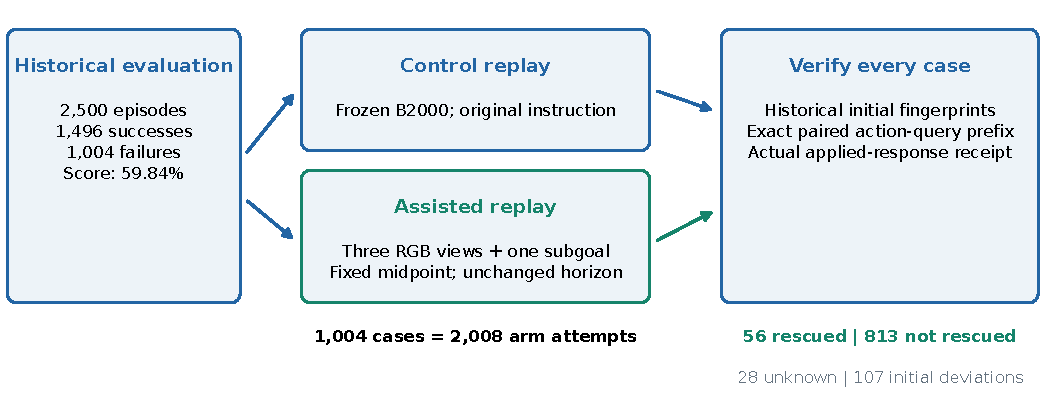
\includegraphics[width=\textwidth]{figures/protocol.pdf}
\caption{\textbf{Two records, one fixed failure cohort.} The original evaluation remains 1,496/2,500. Each of its 1,004 failures is assigned one control and one assisted replay. Assistance changes only the instruction at a fixed query; the robot weights and action horizon remain frozen. Offline replay checks and actual-response evidence determine whether the pair is eligible. All four terminal categories stay in the cohort denominator.}
\label{fig:protocol}
\end{figure*}

\section{Introduction}
\label{sec:intro}
A robot can understand a household instruction yet fail to execute it. After a missed interaction or an unproductive continuation, a vision-language assistant could describe what to do next while a frozen vision-language-action (VLA) policy continues controlling the robot. This interface is appealing because it requires neither policy retraining nor a new motor-action representation. Its value depends on a less obvious question: \emph{does a changed instruction merely change the action output, or does it recover the task?}

Language-mediated planning and recovery are well established~\cite{saycan,innermonologue,reflect,racer,flare}. Here we study a restricted setting that exposes both the opportunity and the limitations of this interface: one image-conditioned instruction, a fixed midpoint trigger, an unchanged robot policy, and the original environment-step budget. The intervention occurs during a fresh replay of a historically failed episode; it does not restart the robot from that episode's terminal failed state. Neither a visible failure nor a hidden simulator failure predicate is required to trigger assistance.

OriginX is a frozen derivative of Xiaomi-Robotics-1-RoboCasa365~\cite{xiaomi}. Its completed 50-task evaluation yields 1,496 successes and 1,004 failures. We retain that historical record and attempt one control and one assisted replay of every failure. Three research questions organize the study: \textbf{RQ1:} How much of this cohort admits a verifiable assisted comparison? \textbf{RQ2:} When advice changes the policy output, how often and how quickly does the task recover? \textbf{RQ3:} Where does recovery remain limited, and what overhead does assistance introduce?

These questions require distinguishing a retry from a comparable intervention. A reset may produce a different initial scene; paired arms may diverge before the instruction changes; generated advice may never reach the policy. Our offline verifier compares historical initial fingerprints, paired preintervention traces, and linked evidence of actual response application. The assistant itself sees only current RGB views, the task instruction, and its remaining action budget. Every historical failure retains a terminal category, including cases whose comparison cannot be validated.

The evidence reveals a gap between output sensitivity and successful recovery. All 869 eligible pairs receive verified advice and produce a different action hash at the first intervention query, where their state and images still match. Only 56 finish the task. Valid-assistance coverage is 86.55\%; multiplying it by the 6.44\% eligible-pair rescue fraction gives the fixed-cohort yield of 5.58\%. Composite-Unseen has the highest coverage but the lowest conditional rescue fraction. Successful cases often finish well after intervention: 29 of 56 finish only after using more than half the remaining budget. Assistance also introduces a median 191-second request wait.

Our contributions are an executed, fully accounted study of 1,004 historical failures; a replay-verification protocol that separates coverage, action-output change, and task recovery; and trace-grounded analyses of recovery timing, task heterogeneity, and inference overhead. The novelty is the empirical characterization under these constraints, not language correction itself. We preserve the 813 eligible non-rescues and 135 unknown or deviating cases. Because historically successful episodes were not revisited and simpler language controls were not run, this study cannot establish deployment-wide improvement or attribute the effect uniquely to Astra's visual reasoning.

\section{Related Work}
\label{sec:related}
\paragraph{Language, feedback, and recovery.}
SayCan grounds language-model plans in robot skill affordances~\cite{saycan}. Inner Monologue feeds environmental feedback into language planning~\cite{innermonologue}. REFLECT summarizes multimodal experience to explain and correct execution failures~\cite{reflect}; RACER studies language-assisted correction and execution~\cite{racer}; FLARE targets failure-aware recovery for long-horizon manipulation~\cite{flare}. RT-H learns language-action hierarchies with correction interfaces~\cite{rth}; CycleVLA uses progress-aware transitions and backtracking~\cite{cyclevla}; ReCoVLA learns residual recovery policies with VLM guidance~\cite{recovla}. These works establish that language-mediated recovery is a developed research direction. OriginX evaluates a deliberately restricted setting: a frozen policy, one scheduled image-conditioned instruction, no iterative assistant feedback, and the original environment-step horizon. Our comparison is with the same unassisted policy. We do not reproduce these systems or claim to outperform them.

\paragraph{Policies and parameter-efficient adaptation.}
Xiaomi-Robotics-1 provides the pretrained visual-language-action model used here~\cite{xiaomi}. Its inherited capabilities dominate the scale of the system. OriginX adds an Action LoRA adapter~\cite{lora} and a small observation-conditioned modulation of the action transformer's adaptive-normalization interface, related to conditional transformer generation~\cite{dit}. Its flow-based action objective follows the released policy rather than introducing a new flow formulation~\cite{flow}. The later assistance study freezes all these components. We separate this policy substrate from the language wrapper because the available experiments do not isolate the contribution of the modulation branch.

\paragraph{Evaluation and experimental comparability.}
RoboCasa and RoboCasa365 support large-scale simulated household manipulation~\cite{robocasa,robocasa365}. We use the documented multi-task setting with pretraining scenes and Atomic-Seen, Composite-Seen, and Composite-Unseen task splits~\cite{protocol}. SIMPLER highlights the importance of carefully specified simulation interfaces when evaluating robot policies~\cite{simpler}. LIBERO-RECOVER constructs a dedicated recovery evaluation from robot failures~\cite{liberorecover}; we do not claim the first recovery benchmark. Our concern is within-study comparability: a seed and task name are not by themselves evidence of equal initial observations or equal preintervention behavior. We retain fingerprints, paired query traces, and intervention receipts alongside terminal outcomes, allowing raw retry success to be distinguished from a verified rescue.

\section{Frozen Policy and Assistance Interface}
\label{sec:method}
\subsection{The OriginX policy substrate}
The frozen endpoint $\policy=\pi_{\theta_0,\alpha,\phi}$ contains the released Xiaomi parameters $\theta_0$, an Action LoRA adapter $\alpha$, and a 4,216,839-parameter observation-conditioned branch $\phi$ that modulates the action transformer's adaptive normalization. Its complete architecture, data lineage, and training losses are documented in the supplement. The assistance experiment updates none of these parameters and supplies no privileged stage labels at inference.

The public adapter alias A2000 refers to unchanged weights trained for 1,613 updates; B2000 identifies the branch after 2,000 updates. This policy substrate is not a separately validated methodological contribution. An earlier 600-pair comparison against the original policy produced 419 versus 413 successes, with 53 B-only and 47 original-only outcomes (exact McNemar $p=0.6173$). It changes both adapter and branch under a different protocol and neither isolates the branch nor supplies a matched baseline for the later 2,500 episodes.

\subsection{A single scheduled language intervention}
The policy replans every 16 environment steps. For horizon $H$, the assistance trigger is
\begin{equation}
\tau=16\left\lceil H/32\right\rceil.
\label{eq:trigger}
\end{equation}
This is the first regular query at or after half the horizon. The trigger depends only on the fixed action budget, not on hidden success state, retrospective failure information, or a learned stall score. The original failure list selects the \emph{study cohort}; its outcome labels are not supplied to the assistant.

At $\tau$, the wrapper sends the original task instruction, current left/right/wrist RGB images (256$\times$256 each), and remaining environment steps to \texttt{gpt-6-astra} at \texttt{high} reasoning effort. Routing identifiers associate each response with its case. Hidden simulator state, success predicates, future frames, and original outcome labels are excluded. The robot policy continues receiving its ordinary proprioceptive observations; these are not additionally sent to Astra.

The supplement reproduces the fixed prompt, response-schema factory, and append rule. The response provides at most 1,500 characters of subgoal text. The wrapper preserves the original instruction, appends ``Immediate next actions:'' and that text, then appends ``Then complete the original task.'' The augmented instruction persists for subsequent policy queries. Astra receives no second observation and produces no motor actions. Its generated rationale is not a verified explanation of failure.

The broker groups at most eight distinct requests into labeled image contact sheets. Each response must pass the recorded schema and identity checks. The prompt forbids tool use, and event traces are checked for tool calls. The CLI invocation records the requested model and reasoning effort; it is not an independently attested identity of service-side model weights. Batch context is a shared resource and a possible source of dependence between cases, not eight separate model invocations.

\subsection{Budget and runtime invariants}
Both arms preserve seed, task, native reset, endpoint, observation history, five Euler integration steps, replanning interval, crop ratio, and registered horizon. Simulation pauses while awaiting assistance, for at most 1,200 wall-clock seconds. This wait consumes additional inference and wall time but does not add action steps. The control is therefore \emph{action-budget matched}, not compute- or latency-matched. Read-only RNG keepalives keep the same policy socket alive without reconnecting or resetting it. Missing, invalid, or unapplied responses remain technical outcomes; completed failures are not rerun to select a better outcome.

\section{Paired Replay Design}
\label{sec:design}
\subsection{Historical record and fixed cohort}
The historical native-reset evaluation contains 50 tasks with 50 episodes each: 18 Atomic-Seen, 16 Composite-Seen, and 16 Composite-Unseen, in pretraining scenes. Environment and policy seeds are fixed in $[2090900000,2090902499]$; task horizons follow RoboCasa 1.0.1. All 2,500 planned episodes have terminal records, with zero missing or infrastructure-unknown outcomes. Every failure reaches its original horizon. The original Counter reset implementation is checked before and after each episode.

We define the rescue cohort before replay as
\begin{equation}
\F=\{i:Y_i^{\mathrm{historical}}=0\},\qquad |\F|=\N.
\end{equation}
It spans 49 tasks; CloseFridge contributes no cases because its historical 50 episodes all succeeded. Each case is assigned two arms, giving 2,008 planned arm attempts but only 1,004 unique cases. The first campaign permanently claims 36 cases; an infrastructure continuation claims the other 968. This partition is fixed at whole-case level before continuation. No later outcome is substituted for a first-partition outcome.

Four infrastructure-development cases, indices 48, 97, 249, and 345, were run separately before the main study and yielded zero pilot rescues. Their pilot outcomes are excluded, but their identities remain in the primary cohort and are explicitly development-exposed. We report a leave-these-identities-out sensitivity analysis rather than describe the full cohort as untouched test data.

\subsection{Verification gates and terminal categories}
\label{sec:gates}
For each case, the verifier checks three distinct conditions. \textbf{Initial agreement} requires both replay initial fingerprints to agree with the historical case, including the recorded scene, observation, instruction, and state evidence. \textbf{Prefix agreement} requires exact paired state/image/instruction/action-query hashes before the intervention. \textbf{Applied assistance} requires linked request, image, response, CLI, and policy-query evidence showing that a valid Astra response actually reached the assisted arm. The state checks are offline measurements; their privileged contents are never policy or assistant inputs.

Let $M_i$ indicate valid completed arms with matching historical initial fingerprints and paired preintervention evidence. Let $A_i$ indicate verified applied assistance and $E_i=M_iA_i$. The rescue indicator is
\begin{equation}
R_i=E_i\ind[Y_i^{C}=0,\ Y_i^{A}=1].
\label{eq:rescue}
\end{equation}
Here $C$ and $A$ denote the control and assisted outcomes. A valid response with no outcome, or an assisted success without matching evidence, is not a strict rescue. An eligible pair that does not satisfy the outcome transition is a non-rescue. Confirmed initial mismatches receive their own deviation category; otherwise missing or invalid evidence remains unknown. These categories are exhaustive and mutually exclusive in the settled ledger.

A further trace audit checks equal state and RGB hashes at the intervention query itself, before the changed instruction is evaluated. The checks strengthen a within-case comparison, but do not prove simulator equivalence outside the recorded contracts. In particular, preintervention traces are compared between the two new arms; they are not reconstructed historical trajectories. The historical archive contains outcome records and initial fingerprints, not videos of the original failures. We cannot retrospectively identify the original first physical error from a hash.

\subsection{Coverage and recovery are different quantities}
The primary estimand is the realized confirmed rescue fraction of the fixed historical cohort, $\widehat r_{\F}=\sum_iR_i/N$, with $N=1004$. Its exact accounting identity is
\begin{equation}
\underbrace{\frac{R}{N}}_{\text{confirmed yield}}
=\underbrace{\frac{E}{N}}_{\text{valid coverage}}\,
\underbrace{\frac{R}{E}}_{\text{conditional recovery}},\qquad E>0.
\label{eq:rates}
\end{equation}
This decomposition distinguishes a missing valid comparison from an observed failure after valid assistance. Unknowns and deviations remain in $N$. The matched-complete count $M$ is an intermediate evidence quantity; $R/M$ is reported in the supplement. Neither $R/E$ nor $R/N$ is an overall deployment success rate. The 1,496 historical successes were not retested, so assistance-induced regressions on them are unmeasured.

The counts form a census of a failure-selected cohort. Task, timing, and batch analyses are retrospective, not preregistered tests. We report technical attrition directly, without assuming missing-at-random outcomes or imputing success. Zero control successes are an observed property of the eligible replays, not an eligibility requirement. The paired asymmetry does not establish full-population improvement.

\section{Results}
\label{sec:results}
\subsection{Baseline performance and the opportunity set}
\begin{table}[t]
\centering\small
\begin{tabular}{@{}lrrr@{}}
\toprule
Historical split & Tasks & Successes & Rate\\
\midrule
Atomic-Seen &18&747/900&83.00\%\\
Composite-Seen &16&479/800&59.88\%\\
Composite-Unseen &16&270/800&33.75\%\\
\midrule
All tasks &50&1496/2500&59.84\%\\
\bottomrule
\end{tabular}
\caption{\textbf{Frozen historical evaluation.} This single-arm record defines the later failure cohort. It is unchanged by assisted replays. Equal trials per task make the pooled rate equal to the task mean.}
\label{tab:baseline}
\end{table}
Table~\ref{tab:baseline} records the frozen endpoint. The 49.25-point Atomic-Seen versus Composite-Unseen gap motivates studying failures, but does not diagnose their causes. Composite-Unseen supplies 530 of the 1,004 failures (52.79\%). GatherTableware, HeatKebabSandwich, and PanTransfer each fail all 50 historical episodes. These failures identify an opportunity set for investigation; they do not establish that an instruction-level correction is sufficient. We omit unmatched leaderboard comparisons because different execution stacks and unavailable paired outcomes prevent attribution of small score differences.

\subsection{RQ1: How much of the cohort is verifiable?}
\begin{table}[t]
\centering\small
\begin{tabular}{@{}lrr@{}}
\toprule
Terminal category & Cases & Fraction of cohort\\
\midrule
Strict rescue &56&5.58\%\\
Eligible non-rescue &813&80.98\%\\
Technical unknown &28&2.79\%\\
Initial-state deviation &107&10.66\%\\
\midrule
Fixed cohort &1004&100.00\%\\
\bottomrule
\end{tabular}
\caption{\textbf{Complete accounting, incomplete valid coverage.} All planned attempts are terminal. Unknowns and deviations are not converted to policy failures or removed from the denominator; rounded percentages need not sum exactly.}
\label{tab:coverage}
\end{table}
Table~\ref{tab:coverage} gives the complete ledger. We obtain $M=874$ matched completed replay pairs and $E=869$ pairs with verified applied assistance. Thus $86.55\%\times6.44\%=5.58\%$ up to rounding: the conditional result alone omits the 13.45\% without a valid intervention comparison. Completed accounting does not mean complete valid coverage.

Among eligible pairs, the complete paired table is 56 assisted-only successes and 813 failures in both arms, with zero control-only and zero both-arm successes. The 874-pair raw matched table adds five both-failure pairs whose assistance evidence is invalid; those five remain unknown, not eligible non-rescues. Their presence illustrates why terminal success bits alone cannot establish that an intervention was tested.

The first partition yields 0 rescues, 3 non-rescues, 28 unknowns, and 5 initial deviations. The continuation yields 56, 810, 0, and 102 respectively. All 28 unknowns therefore arise in the first partition. The continuation changed infrastructure handling, including same-socket keepalives and continued dispatch after validated native-reset deviations. We retain partition membership because this operational history can affect technical coverage. The study is not an uninterrupted homogeneous execution, although its endpoint, action budget, and intervention rule are fixed.

\subsection{RQ2: Does advice change actions and outcomes?}
\label{sec:behavior}
At the intervention query, all 869 eligible pairs have identical recorded state and RGB hashes, different instruction hashes, and immediately different returned action hashes. The action hash covers the returned array's shape, dtype, and bytes; it does not include the instruction. Thus zero-step action-output divergence is observed in all 56 rescued and all 813 non-rescued pairs, with no missing trigger record. This establishes a computational difference, not its magnitude or usefulness. Hashes cannot distinguish a meaningful motor correction from a tiny numerical perturbation, and this comparison does not independently randomize service scheduling or arithmetic effects.

To measure recovery timing, define $u_i=(T_i-\tau_i)/(H_i-\tau_i)$ for a rescued pair, where $T_i$ is its recorded success step. Figure~\ref{fig:timing} plots
\begin{equation}
G_E(u)=\frac{1}{869}\sum_{i:R_i=1}\ind[u_i\leq u],
\end{equation}
with zero contribution from non-rescues. Unlike a CDF conditioned only on success, this curve retains all eligible failures in its denominator and ends at 6.44\%, not 100\%.

\begin{figure}[t]
\centering
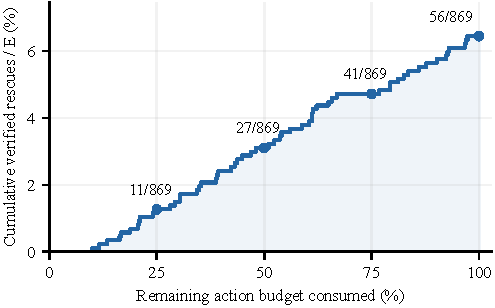
\includegraphics[width=\columnwidth]{figures/recovery_timing.pdf}
\caption{\textbf{Recovery takes continued action.} At 25/50/75/100\% of the remaining budget, 11/27/41/56 cases have succeeded, out of 869 eligible pairs. All 813 eligible non-rescues reach their original horizons. The curve describes recorded success timing, not performance under alternative intervention times.}
\label{fig:timing}
\end{figure}

Among the 56 rescues, median $u_i$ is 51.67\% (interquartile range 30.45--77.41\%), and the median continuation is 361 environment steps. Fifteen rescues finish in the last quarter of their remaining budget; seven use more than 90\%. A short observation window after advice would therefore miss recorded successes. An earlier trigger might help, harm, or leave outcomes unchanged; that counterfactual has not been tested.


\subsection{RQ3: Where does recovery remain limited?}
\begin{table*}[t]
\centering\small
\begin{tabular}{@{}lrrrrrr@{}}
\toprule
Original failure split & Fixed cases & Eligible $E$ & Rescued & Unknown & Initial deviation & Rescued/fixed cases\\
\midrule
Atomic-Seen&153&137&12&0&16&7.84\%\\
Composite-Seen&321&243&25&8&70&7.79\%\\
Composite-Unseen&530&489&19&20&21&3.58\%\\
\midrule
All&1004&869&56&28&107&5.58\%\\
\bottomrule
\end{tabular}
\caption{\textbf{Task familiarity and technical coverage.} Counts are conditioned on historical failure. The lower confirmed rescue fraction in Composite-Unseen is descriptive: the splits have different tasks and horizons, and no controlled generalization effect is identified. In particular, Composite-Seen has a much higher initial-deviation count.}
\label{tab:splits}
\end{table*}
Table~\ref{tab:splits} and Fig.~\ref{fig:coverage} expose two different limitations. Valid coverage is 89.54\%, 75.70\%, and 92.26\% in Atomic-Seen, Composite-Seen, and Composite-Unseen; conditional recovery is 8.76\%, 10.29\%, and 3.89\%. The lowest yield in Composite-Unseen is therefore not the arithmetic consequence of lower coverage. Conversely, Composite-Seen loses 70/321 cases to initial-state deviations, compared with 21/530 in Composite-Unseen. These patterns separate the accounting factors without identifying why the splits differ.

Rescues span 27 of the 49 tasks with historical failures. BreadSelection and PrepareCoffee account for 13/56 rescues (23.21\%); the five largest rescue counts contribute 24/56 (42.86\%). Equal weighting of failure-containing tasks gives 7.83\%, compared with the pooled 5.58\%; these weight different task mixtures. Complete rows are retained in the supplement.

The three originally zero-success tasks yield one rescue in 150 failures (135 eligible pairs); the five lowest historical task scores yield one in 237 (219 eligible). These difficult subsets remain unresolved. However, the full task scatter does not support a monotonic difficulty law: historical task success has descriptive Spearman correlation 0.075 with fixed-cohort yield (49 tasks), and 0.117 with eligible-pair recovery (48 tasks). The bottom-five finding is a retrospective subset description, not a general predictor of recoverability.

Whole-task resampling within original splits gives a 3.59--7.95\% percentile range for confirmed yield. This exploratory task-mixture sensitivity is not a confidence interval for the finite census or a causal effect; its assumptions and the separate batch sensitivity are detailed in the supplement.


\begin{figure*}[t]
\centering
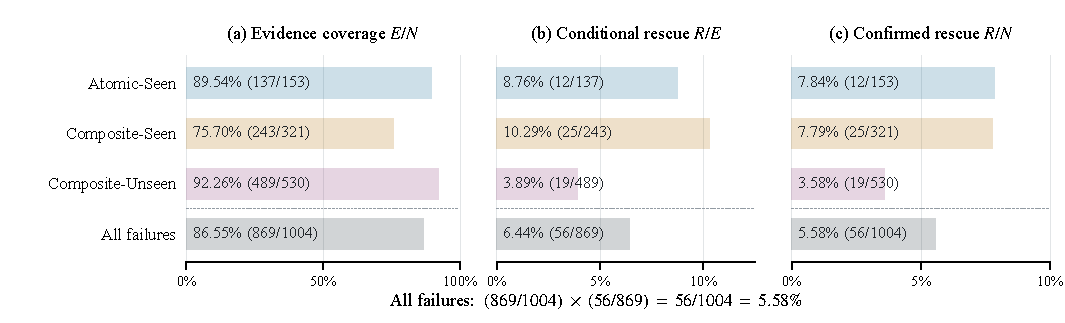
\includegraphics[width=\textwidth]{figures/coverage_recovery.pdf}
\caption{\textbf{Technical coverage and behavioral recovery separate.} Each row factorizes the confirmed yield under Eq.~\ref{eq:rates}. Composite-Unseen has the highest eligible coverage and the lowest conditional rescue fraction. This is a descriptive split comparison, not a controlled effect of task novelty.}
\label{fig:coverage}
\end{figure*}

\subsection{Development exposure sensitivity}
Removing all four pilot case identities leaves 1,000 historical failures with \NoPilotRescues{} rescues, \NoPilotNotRescued{} non-rescues, \NoPilotUnknown{} unknowns, and \NoPilotDeviation{} initial deviations. The confirmed fraction is \NoPilotRate{}\%, compared with 5.58\% in the full cohort. The primary results remain unchanged; this is a transparent sensitivity calculation, not a replacement test population. The pilot's separate 0/4 outcomes are never added to the primary table.

\subsection{Two matched outcomes within the same task}
\begin{figure*}[t]
\centering
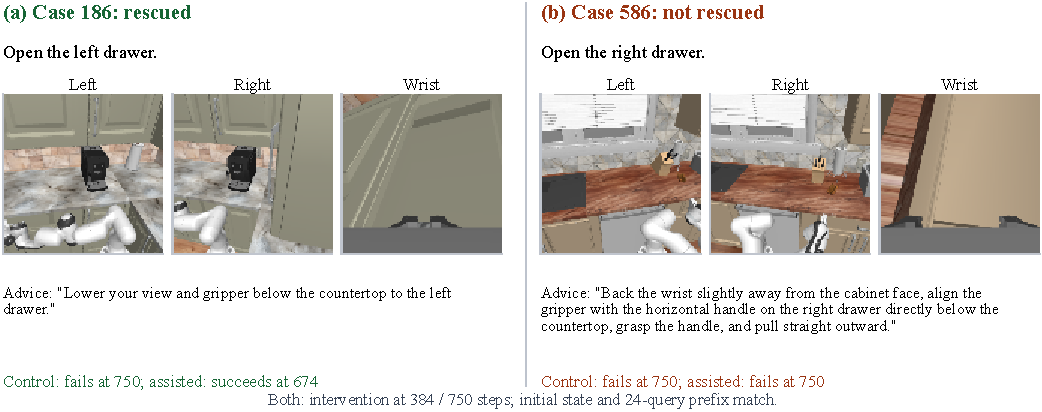
\includegraphics[width=\textwidth]{figures/cases_compact.pdf}
\caption{\textbf{Actual intervention observations for both historical OpenDrawer failures.} The rows show the original three RGB views at the trigger, not reconstructed videos or generated scenes. Both pairs match their historical initial fingerprints and have 24 exact paired preintervention queries; both trigger at step 384 with horizon 750. Case 186 is rescued (assisted success at 674; control fails at 750). Case 586 is not (both fail at 750). These observations and instructions illustrate two outcomes of the same assistance interface; they do not establish a physical causal explanation.}
\label{fig:cases}
\end{figure*}
Figure~\ref{fig:cases} shows the complete two-case historical OpenDrawer failure subset. In case 186 (seed 2090900186), Astra supplies a subgoal about approaching the visible drawer handle, grasping it, and pulling outward. The applied response is linked to the policy's changed instruction. Its assisted arm succeeds at step 674, while the unassisted control exhausts the 750-step horizon. Case 586 (seed 2090900586) also receives valid advice but neither arm succeeds. Equal initial and paired-prefix evidence localizes the experimental difference to the intervention period under the checked contracts. It does not tell us which phrase, visual interpretation, or subsequent physical motion produced the positive outcome; the recorded trigger images are not a postintervention trajectory.

\subsection{Operational cost of the intervention}
\begin{table}[t]
\centering\small
\begin{tabular}{@{}lr@{}}
\toprule
Primary-study accounting & Recorded value\\
\midrule
Unique CLI invocations &135 (134 successful)\\
Known input tokens &2,592,713\\
Known output tokens &195,237\\
Reported reasoning tokens &75,511\\
Median CLI time / invocation &46.16 s\\
Median eligible-case request wait &\WaitMedian{} s\\
95th percentile eligible-case wait &\WaitPninetyfive{} s\\
\bottomrule
\end{tabular}
\caption{\textbf{Actual inference overhead.} Invocations are deduplicated across batches and receipts. One error lacks counters; complete token totals and dollar cost are unknown. Reasoning tokens are not added again to output tokens. Request waiting includes queue/transport time and is distinct from CLI runtime.}
\label{tab:cost}
\end{table}
Table~\ref{tab:cost} separates model-service time from the robot's intervention wait. The known primary invocation latency sums to 6,186.44 seconds, with median 46.16 seconds and range 2.33--77.35 seconds. Batching means neither the sum nor the median is a per-case latency. Recorded eligible-case request waiting is available for \WaitN{} cases, with median \WaitMedian{} seconds and 95th percentile \WaitPninetyfive{} seconds. This subset excludes timed-out and invalid cases; it is not the latency distribution of all requests. The successful OpenDrawer case waits 327.17 seconds even though its batch's CLI time is 48.98 seconds. This difference matters for deployment: unchanged action steps do not imply low-latency recovery.

The separate pilot uses one additional invocation with 19,071 input and 629 output tokens (137 reported reasoning tokens) and 24.35 seconds of CLI time. Failed or unapplied responses are retained in usage, so cost is not restricted to successful rescues. The authenticated CLI quota does not expose a verified monetary bill for this experiment; we do not assume zero cost or infer a price from unrelated APIs.

\section{Interpretation and Limitations}
\label{sec:limits}
\paragraph{Sensitivity is not successful control.}
The action audit shows unequal first-query outputs in every eligible pair. It does not by itself establish semantic use of advice or exclude numerical and service effects; a same-wrapper sham intervention has not been run. A hash may differ because of a small numerical change. The 56 successful paired outcomes provide stronger task-level evidence, while 813 verified applications remain unsuccessful. Accordingly, output differences should not be treated as a demonstrated recovery mechanism without outcome and trajectory validation.

\paragraph{Attribution to the interface, not a unique reasoning mechanism.}
The experimental contrast changes the instruction and adds external inference. It lacks instruction-restatement, fixed generic recovery text, same-budget language-model, and multiple stochastic retries under comparable extra compute. Consequently, it cannot distinguish Astra-specific reasoning from other benefits of extra language conditioning. Nor does it identify the contribution of OriginX's continuous branch. The earlier unsuccessful paired confirmation and absent A-only ablations remain part of the evidence, not objections that can be resolved by a stronger aggregate claim.

\paragraph{Selected cases and replay attrition.}
The cohort is postselected on historical failure. Successes were not revisited, four case identities were used during infrastructure development, and unmatched or invalid pairs comprise 13.45\% of the cohort. Assistance cannot be declared beneficial overall without evaluating a frozen rule on a fresh complete manifest, including episodes it might harm. Exact recorded prefixes help isolate the within-pair intervention period but do not remove selection, possible batch dependence, simulator limitations, or service-version drift. A blinded independent rerun is still needed.

\paragraph{Reproducibility and scope.}
The evidence includes model/configuration identities, case manifests, per-arm outcomes, trace hashes, actual requests/responses, source snapshots, and deduplicated usage. The simulator uses OSMesa with disclosed rendering and context-management changes; query-pixel checks support internal consistency, not universal simulator equivalence. The release's portable loader has CPU contract checks but has not undergone a new real-model GPU parity run. These results cover one policy, one benchmark setting, and one assistance budget. They do not establish real-robot safety, cross-embodiment transfer, or SIMPLER performance. The supplement separates tested contracts from untested portability claims.

\section{Future Directions}
\label{sec:future}
\paragraph{Test visual grounding against simple language controls.}
The highest-priority follow-up is a fresh, sealed complete manifest comparing no intervention, task restatement, fixed generic recovery text, vision-blind assistance, and image-conditioned assistance at the same trigger. The primary contrast is image-conditioned versus vision-blind advice; the simple controls measure what extra text alone accomplishes. A claim that visual grounding adds value requires improved task outcomes in that contrast, not merely different actions. Report paired task-level net success, regressions, coverage, tokens, and waiting time; the action horizon remains fixed, and extra inference is accounted separately. The present evidence does not predict which arm will win.

\paragraph{Test timing and feedback under a fixed resource budget.}
The recovery-time distribution motivates comparing a predeclared trigger grid with the midpoint rule, and then an observation-only trigger learned on separate development episodes. Timing, instruction content, and extra interaction must be varied separately. A closed-loop extension could observe the result of one subgoal before issuing another, but should face the same total token, waiting-time, and action limits as its one-shot comparator. A higher conditional success fraction alone is insufficient if fewer cases receive valid service; report the full coverage--recovery decomposition and latency together.

\paragraph{Distill, replicate, and falsify the proposed mechanism.}
Verified successes can seed a recovery dataset only after the postintervention state-action trajectories are retained and validated; generated instructions alone are not action labels. Keep failed attempts and seal new tasks or seeds before evaluating a distilled policy. Repeating the matched study with another frozen policy, an open assistant, and a second environment would test whether the observed output--outcome gap transfers. Physical trials would additionally require contact, stop, and latency safeguards. Evidence of task gains over text-only controls, repeatability across systems, and acceptable overhead would strengthen the case for deployable language recovery. These are planned tests, not results of this study.

\section{Conclusion}
Matched replay produces different first-intervention action outputs in all 869 valid comparisons, but only 56 task rescues. Fixed-cohort accounting yields 56/1,004 confirmed rescues, retaining 813 non-rescues, 28 unknowns, and 107 initial-state deviations. Coverage, behavioral recovery, continuation budget, and wall-clock latency expose distinct limits of this frozen-policy interface. The original 59.84\% evaluation remains unchanged. The next scientific test is whether visual assistance outperforms simpler text interventions on a fresh complete cohort, including regressions.

{\small% Metadata verified against primary author/proceedings pages on 2026-10-09.
% SayCan uses the PMLR proceedings author order and publication year.
% Xiaomi is credited to the corporate author listed by arXiv.
% Preprints are not assigned unverified conference venues.
\begin{thebibliography}{17}

\bibitem{saycan}
Brian Ichter, Anthony Brohan, Yevgen Chebotar, et~al.
Do As I Can, Not As I Say: Grounding Language in Robotic Affordances.
In \emph{Proceedings of the 6th Conference on Robot Learning}, PMLR 205, pages 287--318, 2023.
\url{https://proceedings.mlr.press/v205/ichter23a.html}.

\bibitem{innermonologue}
Wenlong Huang, Fei Xia, Ted Xiao, Harris Chan, Jacky Liang, Pete Florence, Andy Zeng, Jonathan Tompson, Igor Mordatch, Yevgen Chebotar, Pierre Sermanet, Noah Brown, Tomas Jackson, Linda Luu, Sergey Levine, Karol Hausman, and Brian Ichter.
Inner Monologue: Embodied Reasoning through Planning with Language Models.
\emph{arXiv:2207.05608}, 2022.
\url{https://arxiv.org/abs/2207.05608}.

\bibitem{reflect}
Zeyi Liu, Arpit Bahety, and Shuran Song.
REFLECT: Summarizing Robot Experiences for Failure Explanation and Correction.
In \emph{Proceedings of the 7th Conference on Robot Learning}, PMLR 229, pages 3468--3484, 2023.
\url{https://proceedings.mlr.press/v229/liu23g.html}.

\bibitem{racer}
Yinpei Dai, Jayjun Lee, Nima Fazeli, and Joyce Chai.
RACER: Rich Language-Guided Failure Recovery Policies for Imitation Learning.
\emph{arXiv:2409.14674}, 2024.
\url{https://arxiv.org/abs/2409.14674}.

\bibitem{flare}
Ganlong Zhao, Zijia Tang, Xingping Chen, Zhanghui Kuang, Ye Tian, and Guanbin Li.
FLARE: A Failure-Aware Framework for Autonomous Correction and Recovery in Visual-Language Robotic Manipulation.
In \emph{IEEE/CVF Conference on Computer Vision and Pattern Recognition}, 2026.
\url{https://arxiv.org/abs/2608.26645}.

\bibitem{xiaomi}
Xiaomi Robotics Team.
Xiaomi-Robotics-1: Scaling Vision-Language-Action Models with over 100K Hours of Real-World Trajectories.
\emph{arXiv:2607.15330}, 2026.
\url{https://arxiv.org/abs/2607.15330}.

\bibitem{lora}
Edward J. Hu, Yelong Shen, Phillip Wallis, Zeyuan Allen-Zhu, Yuanzhi Li, Shean Wang, Lu Wang, and Weizhu Chen.
LoRA: Low-Rank Adaptation of Large Language Models.
\emph{arXiv:2106.09685}, 2021.
\url{https://arxiv.org/abs/2106.09685}.

\bibitem{dit}
William Peebles and Saining Xie.
Scalable Diffusion Models with Transformers.
In \emph{IEEE/CVF International Conference on Computer Vision}, pages 4195--4205, 2023.
\url{https://arxiv.org/abs/2212.09748}.

\bibitem{flow}
Yaron Lipman, Ricky T. Q. Chen, Heli Ben-Hamu, Maximilian Nickel, and Matt Le.
Flow Matching for Generative Modeling.
In \emph{International Conference on Learning Representations}, 2023.
\url{https://openreview.net/pdf?id=PqvMRDCJT9t}.

\bibitem{robocasa}
Soroush Nasiriany, Abhiram Maddukuri, Lance Zhang, Adeet Parikh, Aaron Lo, Abhishek Joshi, Ajay Mandlekar, and Yuke Zhu.
RoboCasa: Large-Scale Simulation of Everyday Tasks for Generalist Robots.
In \emph{Robotics: Science and Systems}, 2024.
\url{https://arxiv.org/abs/2406.02523}.

\bibitem{robocasa365}
Soroush Nasiriany, Sepehr Nasiriany, Abhiram Maddukuri, and Yuke Zhu.
RoboCasa365: A Large-Scale Simulation Framework for Training and Benchmarking Generalist Robots.
In \emph{International Conference on Learning Representations}, 2026.
\url{https://robocasa.ai/}.

\bibitem{protocol}
RoboCasa Team.
Multi-Task Learning.
\emph{RoboCasa 1.0.1 Documentation}, accessed October 9, 2026.
\url{https://robocasa.ai/docs/build/html/benchmarking/multitask_learning.html}.

\bibitem{simpler}
Xuanlin Li, Kyle Hsu, Jiayuan Gu, Karl Pertsch, Oier Mees, Homer Rich Walke, Chuyuan Fu, Ishikaa Lunawat, Isabel Sieh, Sean Kirmani, Sergey Levine, Jiajun Wu, Chelsea Finn, Hao Su, Quan Vuong, and Ted Xiao.
Evaluating Real-World Robot Manipulation Policies in Simulation.
\emph{arXiv:2405.05941}, 2024.
\url{https://arxiv.org/abs/2405.05941}.

\bibitem{rth}
Suneel Belkhale, Tianli Ding, Ted Xiao, Pierre Sermanet, Quon Vuong, Jonathan Tompson, Yevgen Chebotar, Debidatta Dwibedi, and Dorsa Sadigh.
RT-H: Action Hierarchies Using Language.
\emph{arXiv:2403.01823}, 2024.
\url{https://arxiv.org/abs/2403.01823}.

\bibitem{cyclevla}
Chenyang Ma, Kai Lu, Guangyu Yang, Jiuming Liu, Shitong Xu, Bill Byrne, Ioannis Havoutis, Niki Trigoni, and Andrew Markham.
CycleVLA: Proactive Self-Correcting Vision-Language-Action Models via Subtask Backtracking and Minimum Bayes Risk Decoding.
\emph{arXiv:2601.02295}, 2026.
\url{https://arxiv.org/abs/2601.02295}.

\bibitem{recovla}
Haodi Hu, Chung-Ta Huang, Jing Liu, Ye Wang, Kei Suzuki, Matthew Brand, and Toshiaki Koike-Akino.
ReCoVLA: VLM-Guided Reward Compilation for Failure Recovery in Vision-Language-Action Policies.
\emph{arXiv:2606.09630}, 2026.
\url{https://arxiv.org/abs/2606.09630}.

\bibitem{liberorecover}
Lin Liu, Zhicheng Bao, Lu Zhang, Ziying Song, Wu Yang, Yuzheng Zhuang, Shuai Tao, Wulong Liu, Caiyan Jia, and Huchuan Lu.
LIBERO-RECOVER: Beyond Task Success Towards Failure Recovery in Robotic Manipulation Models.
\emph{arXiv:2609.05178}, 2026.
\url{https://arxiv.org/abs/2609.05178}.

\end{thebibliography}
}
\end{document}
